\cajita{Tasa de alfabetismo en la población de 15 años o más por sexo, según grupos de edado}{La tasa de alfabetismo en Guatemala se calcula como la población de 15 años o más que reportaron saber leer y escribir sobre el total de dicha población.

Del año 2018 al 2022 se muestra un incremento de 2.8 puntos porcentuales en la tasa de alfabetización de mujeres entre 15 y 29 años. De igual manera, se observa un aumento de 6.4 puntos porcentuales para mujeres entre 30 y 64 años, y un incremanto 1.0 puntos porcentuales para mujeres de 65 años en adelante. }{Tasa de alfabetismo en la población de 15 años o más por sexo, grupos de edad}{República de Guatemala, Instituto Nacional de Estadística}{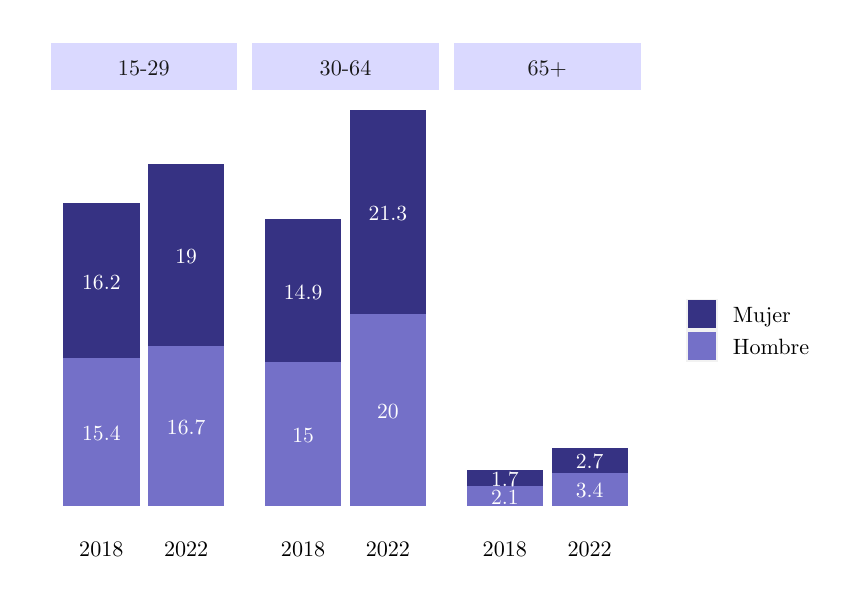
\begin{tikzpicture}[x=1pt,y=1pt]% Created by tikzDevice version 0.12.4 on 2023-05-10 12:05:57
% !TEX encoding = UTF-8 Unicode
\definecolor{fillColor}{RGB}{255,255,255}
\path[use as bounding box,fill=fillColor,fill opacity=0.00] (0,0) rectangle (289.08,198.74);
\begin{scope}
\path[clip] (  0.00,  0.00) rectangle (289.08,198.74);
\definecolor{drawColor}{RGB}{255,255,255}
\definecolor{fillColor}{RGB}{255,255,255}

\path[draw=drawColor,line width= 0.6pt,line join=round,line cap=round,fill=fillColor] (  0.00,  0.00) rectangle (289.08,198.74);
\end{scope}
\begin{scope}
\path[clip] (  0.00,  0.00) rectangle (289.08,198.74);
\definecolor{fillColor}{RGB}{54,50,131}

\path[fill=fillColor] ( 12.85, 79.26) rectangle ( 40.42,135.36);
\definecolor{fillColor}{RGB}{116,112,200}

\path[fill=fillColor] ( 12.85, 25.96) rectangle ( 40.42, 79.26);
\definecolor{fillColor}{RGB}{54,50,131}

\path[fill=fillColor] ( 43.48, 83.67) rectangle ( 71.06,149.33);
\definecolor{fillColor}{RGB}{116,112,200}

\path[fill=fillColor] ( 43.48, 25.96) rectangle ( 71.06, 83.67);
\definecolor{drawColor}{RGB}{255,255,255}

\node[text=drawColor,anchor=base,inner sep=0pt, outer sep=0pt, scale=  0.78] at ( 26.63,104.28) {16.2};

\node[text=drawColor,anchor=base,inner sep=0pt, outer sep=0pt, scale=  0.78] at ( 26.63, 49.57) {15.4};

\node[text=drawColor,anchor=base,inner sep=0pt, outer sep=0pt, scale=  0.78] at ( 57.27,113.47) {19};

\node[text=drawColor,anchor=base,inner sep=0pt, outer sep=0pt, scale=  0.78] at ( 57.27, 51.78) {16.7};
\end{scope}
\begin{scope}
\path[clip] (  0.00,  0.00) rectangle (289.08,198.74);
\definecolor{fillColor}{RGB}{54,50,131}

\path[fill=fillColor] ( 85.75, 77.95) rectangle (113.32,129.49);
\definecolor{fillColor}{RGB}{116,112,200}

\path[fill=fillColor] ( 85.75, 25.96) rectangle (113.32, 77.95);
\definecolor{fillColor}{RGB}{54,50,131}

\path[fill=fillColor] (116.38, 95.16) rectangle (143.96,168.94);
\definecolor{fillColor}{RGB}{116,112,200}

\path[fill=fillColor] (116.38, 25.96) rectangle (143.96, 95.16);
\definecolor{drawColor}{RGB}{255,255,255}

\node[text=drawColor,anchor=base,inner sep=0pt, outer sep=0pt, scale=  0.78] at ( 99.53,100.69) {14.9};

\node[text=drawColor,anchor=base,inner sep=0pt, outer sep=0pt, scale=  0.78] at ( 99.53, 48.92) {15};

\node[text=drawColor,anchor=base,inner sep=0pt, outer sep=0pt, scale=  0.78] at (130.17,129.02) {21.3};

\node[text=drawColor,anchor=base,inner sep=0pt, outer sep=0pt, scale=  0.78] at (130.17, 57.53) {20};
\end{scope}
\begin{scope}
\path[clip] (  0.00,  0.00) rectangle (289.08,198.74);
\definecolor{fillColor}{RGB}{54,50,131}

\path[fill=fillColor] (158.65, 33.08) rectangle (186.22, 38.96);
\definecolor{fillColor}{RGB}{116,112,200}

\path[fill=fillColor] (158.65, 25.96) rectangle (186.22, 33.08);
\definecolor{fillColor}{RGB}{54,50,131}

\path[fill=fillColor] (189.29, 37.76) rectangle (216.86, 47.01);
\definecolor{fillColor}{RGB}{116,112,200}

\path[fill=fillColor] (189.29, 25.96) rectangle (216.86, 37.76);
\definecolor{drawColor}{RGB}{255,255,255}

\node[text=drawColor,anchor=base,inner sep=0pt, outer sep=0pt, scale=  0.78] at (172.44, 32.98) {1.7};

\node[text=drawColor,anchor=base,inner sep=0pt, outer sep=0pt, scale=  0.78] at (172.44, 26.48) {2.1};

\node[text=drawColor,anchor=base,inner sep=0pt, outer sep=0pt, scale=  0.78] at (203.07, 39.35) {2.7};

\node[text=drawColor,anchor=base,inner sep=0pt, outer sep=0pt, scale=  0.78] at (203.07, 28.83) {3.4};
\end{scope}
\begin{scope}
\path[clip] (  0.00,  0.00) rectangle (289.08,198.74);
\definecolor{fillColor}{RGB}{218,217,255}

\path[fill=fillColor] (  8.25,176.08) rectangle ( 75.65,193.24);
\definecolor{drawColor}{gray}{0.10}

\node[text=drawColor,anchor=base,inner sep=0pt, outer sep=0pt, scale=  0.80] at ( 41.95,181.54) {15-29};
\end{scope}
\begin{scope}
\path[clip] (  0.00,  0.00) rectangle (289.08,198.74);
\definecolor{fillColor}{RGB}{218,217,255}

\path[fill=fillColor] ( 81.15,176.08) rectangle (148.55,193.24);
\definecolor{drawColor}{gray}{0.10}

\node[text=drawColor,anchor=base,inner sep=0pt, outer sep=0pt, scale=  0.80] at (114.85,181.54) {30-64};
\end{scope}
\begin{scope}
\path[clip] (  0.00,  0.00) rectangle (289.08,198.74);
\definecolor{fillColor}{RGB}{218,217,255}

\path[fill=fillColor] (154.05,176.08) rectangle (221.46,193.24);
\definecolor{drawColor}{gray}{0.10}

\node[text=drawColor,anchor=base,inner sep=0pt, outer sep=0pt, scale=  0.80] at (187.75,181.54) {65+};
\end{scope}
\begin{scope}
\path[clip] (  0.00,  0.00) rectangle (289.08,198.74);
\definecolor{drawColor}{RGB}{0,0,0}

\node[text=drawColor,anchor=base,inner sep=0pt, outer sep=0pt, scale=  0.80] at ( 26.63,  7.60) {2018};

\node[text=drawColor,anchor=base,inner sep=0pt, outer sep=0pt, scale=  0.80] at ( 57.27,  7.60) {2022};
\end{scope}
\begin{scope}
\path[clip] (  0.00,  0.00) rectangle (289.08,198.74);
\definecolor{drawColor}{RGB}{0,0,0}

\node[text=drawColor,anchor=base,inner sep=0pt, outer sep=0pt, scale=  0.80] at ( 99.53,  7.60) {2018};

\node[text=drawColor,anchor=base,inner sep=0pt, outer sep=0pt, scale=  0.80] at (130.17,  7.60) {2022};
\end{scope}
\begin{scope}
\path[clip] (  0.00,  0.00) rectangle (289.08,198.74);
\definecolor{drawColor}{RGB}{0,0,0}

\node[text=drawColor,anchor=base,inner sep=0pt, outer sep=0pt, scale=  0.80] at (172.44,  7.60) {2018};

\node[text=drawColor,anchor=base,inner sep=0pt, outer sep=0pt, scale=  0.80] at (203.07,  7.60) {2022};
\end{scope}
\begin{scope}
\path[clip] (  0.00,  0.00) rectangle (289.08,198.74);
\definecolor{fillColor}{RGB}{255,255,255}

\path[fill=fillColor] (232.46, 72.59) rectangle (283.58,122.30);
\end{scope}
\begin{scope}
\path[clip] (  0.00,  0.00) rectangle (289.08,198.74);
\definecolor{fillColor}{gray}{0.95}

\path[fill=fillColor] (237.96, 89.47) rectangle (249.34,100.85);
\end{scope}
\begin{scope}
\path[clip] (  0.00,  0.00) rectangle (289.08,198.74);
\definecolor{fillColor}{RGB}{54,50,131}

\path[fill=fillColor] (238.62, 90.14) rectangle (248.67,100.19);
\end{scope}
\begin{scope}
\path[clip] (  0.00,  0.00) rectangle (289.08,198.74);
\definecolor{fillColor}{gray}{0.95}

\path[fill=fillColor] (237.96, 78.09) rectangle (249.34, 89.47);
\end{scope}
\begin{scope}
\path[clip] (  0.00,  0.00) rectangle (289.08,198.74);
\definecolor{fillColor}{RGB}{116,112,200}

\path[fill=fillColor] (238.62, 78.75) rectangle (248.67, 88.81);
\end{scope}
\begin{scope}
\path[clip] (  0.00,  0.00) rectangle (289.08,198.74);
\definecolor{drawColor}{RGB}{0,0,0}

\node[text=drawColor,anchor=base west,inner sep=0pt, outer sep=0pt, scale=  0.80] at (254.84, 92.04) {Mujer};
\end{scope}
\begin{scope}
\path[clip] (  0.00,  0.00) rectangle (289.08,198.74);
\definecolor{drawColor}{RGB}{0,0,0}

\node[text=drawColor,anchor=base west,inner sep=0pt, outer sep=0pt, scale=  0.80] at (254.84, 80.66) {Hombre};
\end{scope}
\end{tikzpicture}}{INE - ENEI 2022, ENEI 2 2018}{}

\cajita{Tasa de alfabetismo en la población de 15 años o más por sexo, según dominio de estudio}{Del año 2018 al 2022 se muestra un incremento de 2.6 puntos porcentuales en la tasa de alfabetización de mujeres en el dominio urbano metropolitano. De igual manera, se observa un aumento de 1.0 puntos porcentuales para mujeres en el resto urbano, y un incremanto 6.5 puntos porcentuales para mujeres en el dominio rural nacional. }{Tasa de alfabetismo en la población de 15 años o más por sexo, según dominio de estudio}{República de Guatemala, Instituto Nacional de Estadística}{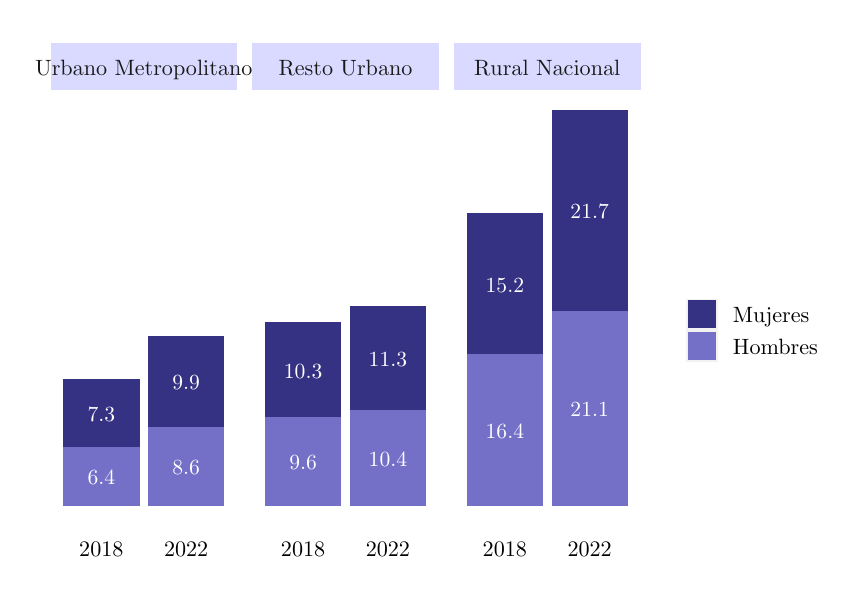
\begin{tikzpicture}[x=1pt,y=1pt]% Created by tikzDevice version 0.12.4 on 2023-05-10 12:06:09
% !TEX encoding = UTF-8 Unicode
\definecolor{fillColor}{RGB}{255,255,255}
\path[use as bounding box,fill=fillColor,fill opacity=0.00] (0,0) rectangle (289.08,198.74);
\begin{scope}
\path[clip] (  0.00,  0.00) rectangle (289.08,198.74);
\definecolor{drawColor}{RGB}{255,255,255}
\definecolor{fillColor}{RGB}{255,255,255}

\path[draw=drawColor,line width= 0.6pt,line join=round,line cap=round,fill=fillColor] (  0.00,  0.00) rectangle (289.08,198.74);
\end{scope}
\begin{scope}
\path[clip] (  0.00,  0.00) rectangle (289.08,198.74);
\definecolor{fillColor}{RGB}{54,50,131}

\path[fill=fillColor] ( 12.85, 47.35) rectangle ( 40.42, 71.61);
\definecolor{fillColor}{RGB}{116,112,200}

\path[fill=fillColor] ( 12.85, 25.96) rectangle ( 40.42, 47.35);
\definecolor{fillColor}{RGB}{54,50,131}

\path[fill=fillColor] ( 43.48, 54.56) rectangle ( 71.06, 87.47);
\definecolor{fillColor}{RGB}{116,112,200}

\path[fill=fillColor] ( 43.48, 25.96) rectangle ( 71.06, 54.56);
\definecolor{drawColor}{RGB}{255,255,255}

\node[text=drawColor,anchor=base,inner sep=0pt, outer sep=0pt, scale=  0.78] at ( 26.63, 56.45) {7.3};

\node[text=drawColor,anchor=base,inner sep=0pt, outer sep=0pt, scale=  0.78] at ( 26.63, 33.62) {6.4};

\node[text=drawColor,anchor=base,inner sep=0pt, outer sep=0pt, scale=  0.78] at ( 57.27, 67.98) {9.9};

\node[text=drawColor,anchor=base,inner sep=0pt, outer sep=0pt, scale=  0.78] at ( 57.27, 37.23) {8.6};
\end{scope}
\begin{scope}
\path[clip] (  0.00,  0.00) rectangle (289.08,198.74);
\definecolor{fillColor}{RGB}{54,50,131}

\path[fill=fillColor] ( 85.75, 58.03) rectangle (113.32, 92.32);
\definecolor{fillColor}{RGB}{116,112,200}

\path[fill=fillColor] ( 85.75, 25.96) rectangle (113.32, 58.03);
\definecolor{fillColor}{RGB}{54,50,131}

\path[fill=fillColor] (116.38, 60.51) rectangle (143.96, 98.34);
\definecolor{fillColor}{RGB}{116,112,200}

\path[fill=fillColor] (116.38, 25.96) rectangle (143.96, 60.51);
\definecolor{drawColor}{RGB}{255,255,255}

\node[text=drawColor,anchor=base,inner sep=0pt, outer sep=0pt, scale=  0.78] at ( 99.53, 72.14) {10.3};

\node[text=drawColor,anchor=base,inner sep=0pt, outer sep=0pt, scale=  0.78] at ( 99.53, 38.96) {9.6};

\node[text=drawColor,anchor=base,inner sep=0pt, outer sep=0pt, scale=  0.78] at (130.17, 76.39) {11.3};

\node[text=drawColor,anchor=base,inner sep=0pt, outer sep=0pt, scale=  0.78] at (130.17, 40.20) {10.4};
\end{scope}
\begin{scope}
\path[clip] (  0.00,  0.00) rectangle (289.08,198.74);
\definecolor{fillColor}{RGB}{54,50,131}

\path[fill=fillColor] (158.65, 80.79) rectangle (186.22,131.61);
\definecolor{fillColor}{RGB}{116,112,200}

\path[fill=fillColor] (158.65, 25.96) rectangle (186.22, 80.79);
\definecolor{fillColor}{RGB}{54,50,131}

\path[fill=fillColor] (189.29, 96.44) rectangle (216.86,168.94);
\definecolor{fillColor}{RGB}{116,112,200}

\path[fill=fillColor] (189.29, 25.96) rectangle (216.86, 96.44);
\definecolor{drawColor}{RGB}{255,255,255}

\node[text=drawColor,anchor=base,inner sep=0pt, outer sep=0pt, scale=  0.78] at (172.44,103.17) {15.2};

\node[text=drawColor,anchor=base,inner sep=0pt, outer sep=0pt, scale=  0.78] at (172.44, 50.34) {16.4};

\node[text=drawColor,anchor=base,inner sep=0pt, outer sep=0pt, scale=  0.78] at (203.07,129.65) {21.7};

\node[text=drawColor,anchor=base,inner sep=0pt, outer sep=0pt, scale=  0.78] at (203.07, 58.17) {21.1};
\end{scope}
\begin{scope}
\path[clip] (  0.00,  0.00) rectangle (289.08,198.74);
\definecolor{fillColor}{RGB}{218,217,255}

\path[fill=fillColor] (  8.25,176.08) rectangle ( 75.65,193.24);
\definecolor{drawColor}{gray}{0.10}

\node[text=drawColor,anchor=base,inner sep=0pt, outer sep=0pt, scale=  0.80] at ( 41.95,181.54) {Urbano Metropolitano};
\end{scope}
\begin{scope}
\path[clip] (  0.00,  0.00) rectangle (289.08,198.74);
\definecolor{fillColor}{RGB}{218,217,255}

\path[fill=fillColor] ( 81.15,176.08) rectangle (148.55,193.24);
\definecolor{drawColor}{gray}{0.10}

\node[text=drawColor,anchor=base,inner sep=0pt, outer sep=0pt, scale=  0.80] at (114.85,181.54) {Resto Urbano};
\end{scope}
\begin{scope}
\path[clip] (  0.00,  0.00) rectangle (289.08,198.74);
\definecolor{fillColor}{RGB}{218,217,255}

\path[fill=fillColor] (154.05,176.08) rectangle (221.46,193.24);
\definecolor{drawColor}{gray}{0.10}

\node[text=drawColor,anchor=base,inner sep=0pt, outer sep=0pt, scale=  0.80] at (187.75,181.54) {Rural Nacional};
\end{scope}
\begin{scope}
\path[clip] (  0.00,  0.00) rectangle (289.08,198.74);
\definecolor{drawColor}{RGB}{0,0,0}

\node[text=drawColor,anchor=base,inner sep=0pt, outer sep=0pt, scale=  0.80] at ( 26.63,  7.60) {2018};

\node[text=drawColor,anchor=base,inner sep=0pt, outer sep=0pt, scale=  0.80] at ( 57.27,  7.60) {2022};
\end{scope}
\begin{scope}
\path[clip] (  0.00,  0.00) rectangle (289.08,198.74);
\definecolor{drawColor}{RGB}{0,0,0}

\node[text=drawColor,anchor=base,inner sep=0pt, outer sep=0pt, scale=  0.80] at ( 99.53,  7.60) {2018};

\node[text=drawColor,anchor=base,inner sep=0pt, outer sep=0pt, scale=  0.80] at (130.17,  7.60) {2022};
\end{scope}
\begin{scope}
\path[clip] (  0.00,  0.00) rectangle (289.08,198.74);
\definecolor{drawColor}{RGB}{0,0,0}

\node[text=drawColor,anchor=base,inner sep=0pt, outer sep=0pt, scale=  0.80] at (172.44,  7.60) {2018};

\node[text=drawColor,anchor=base,inner sep=0pt, outer sep=0pt, scale=  0.80] at (203.07,  7.60) {2022};
\end{scope}
\begin{scope}
\path[clip] (  0.00,  0.00) rectangle (289.08,198.74);
\definecolor{fillColor}{RGB}{255,255,255}

\path[fill=fillColor] (232.46, 72.59) rectangle (283.58,122.30);
\end{scope}
\begin{scope}
\path[clip] (  0.00,  0.00) rectangle (289.08,198.74);
\definecolor{fillColor}{gray}{0.95}

\path[fill=fillColor] (237.96, 89.47) rectangle (249.34,100.85);
\end{scope}
\begin{scope}
\path[clip] (  0.00,  0.00) rectangle (289.08,198.74);
\definecolor{fillColor}{RGB}{54,50,131}

\path[fill=fillColor] (238.62, 90.14) rectangle (248.67,100.19);
\end{scope}
\begin{scope}
\path[clip] (  0.00,  0.00) rectangle (289.08,198.74);
\definecolor{fillColor}{gray}{0.95}

\path[fill=fillColor] (237.96, 78.09) rectangle (249.34, 89.47);
\end{scope}
\begin{scope}
\path[clip] (  0.00,  0.00) rectangle (289.08,198.74);
\definecolor{fillColor}{RGB}{116,112,200}

\path[fill=fillColor] (238.62, 78.75) rectangle (248.67, 88.81);
\end{scope}
\begin{scope}
\path[clip] (  0.00,  0.00) rectangle (289.08,198.74);
\definecolor{drawColor}{RGB}{0,0,0}

\node[text=drawColor,anchor=base west,inner sep=0pt, outer sep=0pt, scale=  0.80] at (254.84, 92.04) {Mujeres};
\end{scope}
\begin{scope}
\path[clip] (  0.00,  0.00) rectangle (289.08,198.74);
\definecolor{drawColor}{RGB}{0,0,0}

\node[text=drawColor,anchor=base west,inner sep=0pt, outer sep=0pt, scale=  0.80] at (254.84, 80.66) {Hombres};
\end{scope}
\end{tikzpicture}}{INE - ENEI 2022, ENEI 2 2018}{}

\cajita{Nivel educativo de la población de 15 años o más por sexo}{La tabla muestra la desagregación de la población de 15 años o más por sexo según el nivel educativo en el cual se reportó su último grado aprobado. 

En ambos años 2018 y 2022, se reportó un mayor porcentaje de mujeres que hombres sin ningún grado aprobado en ningún nivel educativo respectivamente; en esta misma categoría, el porcentaje de mujeres incrementó de 2.5 puntos porcentuales de 2018 a 2022. 

Para 2022, el porcentaje de mujeres con algún grado aprobado en primaria o en diversificado fue mayor que los porcentajes de hombres respectivos. Similarmente, del 2018 al 2022 se reportó un aumento de dichas poblaciones de mujeres, 3.6 puntos porcentuales para primaria y 2.8 para diversificado. }{Nivel educativo de la población de 15 años o más por sexo (porcentaje)}{República de Guatemala, Instituto Nacional de Estadística}{\begin{tabular}[t]{ccccc}
\toprule
\multicolumn{1}{c}{\textbf{ }} & \multicolumn{2}{c}{\textbf{2018}} & \multicolumn{2}{c}{\textbf{2022}} \\
\cmidrule(l{3pt}r{3pt}){2-3} \cmidrule(l{3pt}r{3pt}){4-5}
\textbf{Nivel Educativo} & \textbf{Mujeres} & \textbf{Hombres} & \textbf{Mujeres} & \textbf{Hombres}\\
\midrule
\cellcolor[HTML]{B6B3FF}{Ninguno} & \cellcolor[HTML]{B6B3FF}{9.9} & \cellcolor[HTML]{B6B3FF}{5.0} & \cellcolor[HTML]{B6B3FF}{12.4} & \cellcolor[HTML]{B6B3FF}{6.2}\\
Preprimaria & 0.1 & 0.1 & 0.9 & 0.7\\
\cellcolor[HTML]{B6B3FF}{Primaria} & \cellcolor[HTML]{B6B3FF}{16.2} & \cellcolor[HTML]{B6B3FF}{15.5} & \cellcolor[HTML]{B6B3FF}{19.8} & \cellcolor[HTML]{B6B3FF}{17.0}\\
Básico & 6.0 & 6.4 & 7.7 & 8.5\\
\cellcolor[HTML]{B6B3FF}{Diversificado} & \cellcolor[HTML]{B6B3FF}{7.6} & \cellcolor[HTML]{B6B3FF}{7.6} & \cellcolor[HTML]{B6B3FF}{10.4} & \cellcolor[HTML]{B6B3FF}{9.3}\\
Superior & 2.2 & 2.2 & 3.2 & 3.4\\
\cellcolor[HTML]{B6B3FF}{Posgrado} & \cellcolor[HTML]{B6B3FF}{0.1} & \cellcolor[HTML]{B6B3FF}{0.1} & \cellcolor[HTML]{B6B3FF}{0.3} & \cellcolor[HTML]{B6B3FF}{0.3}\\
\bottomrule
\end{tabular}
}{INE - ENEI 2022, ENEI 2 2018}{}

\cajita{Tasa neta de escolaridad en el nivel primario por sexo}{La tasa neta de escolaridad es la relación porcentual entre el alumnado de la edad tradicional de completación del nivel educativo sobre el total de la población de esa edad.

La gráfica muestra que en Guatemala, la tasa neta de escolaridad en el nivel primario de mujeres sobrepasó la de los hombres en 2020 y 2021. Entre 2018 y 2021, la tasa aumentó en 2.1 puntos porcentuales para las mujeres.}{Tasa neta de escolaridad en el nivel primario por sexo (porcentaje)}{República de Guatemala, Instituto Nacional de Estadística}{\begin{tikzpicture}[x=1pt,y=1pt]% Created by tikzDevice version 0.12.4 on 2023-05-16 13:44:19
% !TEX encoding = UTF-8 Unicode
\definecolor{fillColor}{RGB}{255,255,255}
\path[use as bounding box,fill=fillColor,fill opacity=0.00] (0,0) rectangle (289.08,198.74);
\begin{scope}
\path[clip] (  0.00,  0.00) rectangle (289.08,198.74);

\path[] (  0.00,  0.00) rectangle (289.08,198.74);
\end{scope}
\begin{scope}
\path[clip] (  0.00,  0.00) rectangle (289.08,198.74);
\definecolor{drawColor}{RGB}{54,50,131}

\path[draw=drawColor,line width= 1.7pt,line join=round] ( 39.63, 46.16) --
	(106.55,161.67) --
	(173.47,131.66) --
	(240.39,118.13);
\definecolor{drawColor}{RGB}{116,112,200}

\path[draw=drawColor,line width= 1.7pt,line join=round] ( 39.63, 46.24) --
	(106.55,160.83) --
	(173.47,121.63) --
	(240.39, 94.00);
\definecolor{drawColor}{RGB}{0,0,0}

\node[text=drawColor,anchor=base,inner sep=0pt, outer sep=0pt, scale=  1.02] at ( 39.63, 34.25) {90.2};

\node[text=drawColor,anchor=base,inner sep=0pt, outer sep=0pt, scale=  1.02] at (106.55,165.64) {95.2};

\node[text=drawColor,anchor=base west,inner sep=0pt, outer sep=0pt, scale=  1.02] at (173.47,135.63) {93.9};

\node[text=drawColor,anchor=base,inner sep=0pt, outer sep=0pt, scale=  1.02] at (240.39,106.21) {93.3};

\node[text=drawColor,anchor=base,inner sep=0pt, outer sep=0pt, scale=  1.02] at ( 39.63, 34.32) {90.2};

\node[text=drawColor,anchor=base,inner sep=0pt, outer sep=0pt, scale=  1.02] at (106.55,164.80) {95.2};

\node[text=drawColor,anchor=base west,inner sep=0pt, outer sep=0pt, scale=  1.02] at (173.47,125.60) {93.5};

\node[text=drawColor,anchor=base,inner sep=0pt, outer sep=0pt, scale=  1.02] at (240.39, 82.08) {92.3};

\path[draw=drawColor,line width= 0.1pt,line join=round] (-281.58, 23.41) -- (561.61, 23.41);

\path[] ( -0.52, 15.40) rectangle (280.54,191.63);

\path[] ( -0.52, 41.72) --
	(280.54, 41.72);

\path[] ( -0.52, 87.49) --
	(280.54, 87.49);

\path[] ( -0.52,133.27) --
	(280.54,133.27);

\path[] ( -0.52,179.04) --
	(280.54,179.04);

\path[] ( -0.52, 18.83) --
	(280.54, 18.83);

\path[] ( -0.52, 64.60) --
	(280.54, 64.60);

\path[] ( -0.52,110.38) --
	(280.54,110.38);

\path[] ( -0.52,156.15) --
	(280.54,156.15);

\path[] ( 39.63, 15.40) --
	( 39.63,191.63);

\path[] (106.55, 15.40) --
	(106.55,191.63);

\path[] (173.47, 15.40) --
	(173.47,191.63);

\path[] (240.39, 15.40) --
	(240.39,191.63);

\path[] ( -0.52, 15.40) rectangle (280.54,191.63);
\end{scope}
\begin{scope}
\path[clip] (  0.00,  0.00) rectangle (289.08,198.74);

\path[] ( -0.52, 15.40) --
	( -0.52,191.63);
\end{scope}
\begin{scope}
\path[clip] (  0.00,  0.00) rectangle (289.08,198.74);
\definecolor{drawColor}{RGB}{255,255,255}

\node[text=drawColor,text opacity=0.00,anchor=base east,inner sep=0pt, outer sep=0pt, scale=  1.00] at ( -5.47, 14.92) {89};

\node[text=drawColor,text opacity=0.00,anchor=base east,inner sep=0pt, outer sep=0pt, scale=  1.00] at ( -5.47, 60.70) {91};

\node[text=drawColor,text opacity=0.00,anchor=base east,inner sep=0pt, outer sep=0pt, scale=  1.00] at ( -5.47,106.47) {93};

\node[text=drawColor,text opacity=0.00,anchor=base east,inner sep=0pt, outer sep=0pt, scale=  1.00] at ( -5.47,152.25) {95};
\end{scope}
\begin{scope}
\path[clip] (  0.00,  0.00) rectangle (289.08,198.74);

\path[] ( -3.27, 18.83) --
	( -0.52, 18.83);

\path[] ( -3.27, 64.60) --
	( -0.52, 64.60);

\path[] ( -3.27,110.38) --
	( -0.52,110.38);

\path[] ( -3.27,156.15) --
	( -0.52,156.15);
\end{scope}
\begin{scope}
\path[clip] (  0.00,  0.00) rectangle (289.08,198.74);

\path[] ( -0.52, 15.40) --
	(280.54, 15.40);
\end{scope}
\begin{scope}
\path[clip] (  0.00,  0.00) rectangle (289.08,198.74);

\path[] ( 39.63, 12.65) --
	( 39.63, 15.40);

\path[] (106.55, 12.65) --
	(106.55, 15.40);

\path[] (173.47, 12.65) --
	(173.47, 15.40);

\path[] (240.39, 12.65) --
	(240.39, 15.40);
\end{scope}
\begin{scope}
\path[clip] (  0.00,  0.00) rectangle (289.08,198.74);
\definecolor{drawColor}{RGB}{0,0,0}

\node[text=drawColor,anchor=base,inner sep=0pt, outer sep=0pt, scale=  1.00] at ( 39.63,  1.32) {2018};

\node[text=drawColor,anchor=base,inner sep=0pt, outer sep=0pt, scale=  1.00] at (106.55,  1.32) {2019};

\node[text=drawColor,anchor=base,inner sep=0pt, outer sep=0pt, scale=  1.00] at (173.47,  1.32) {2020};

\node[text=drawColor,anchor=base,inner sep=0pt, outer sep=0pt, scale=  1.00] at (240.39,  1.32) {2021};
\end{scope}
\begin{scope}
\path[clip] (  0.00,  0.00) rectangle (289.08,198.74);
\coordinate (apoyo) at (58.34,189.21);
\coordinate (longitudFicticia) at (7.11,9.53);
\coordinate (longitud) at (7.11,7.11);
\coordinate (desX) at (134.96,0);
\coordinate (desY) at (0,1.21);
\definecolor[named]{ct1}{HTML}{
363283
}
\definecolor[named]{ct2}{HTML}{
7470C8
}
\definecolor[named]{ctb1}{HTML}{
363283
}
\definecolor[named]{ctb2}{HTML}{
7470C8
}
\path [fill=none] (apoyo) rectangle ($(apoyo)+(longitudFicticia)$)
node [xshift=0.3cm,inner sep=0pt, outer sep=0pt,midway,right,scale = 1]{Mujer};
\draw [color = ctb1,fill=ct1] ( $(apoyo)  + (desY) $) rectangle ($(apoyo)+ (desY) +(longitud)$);
\path [fill=none] ($(apoyo)+(desX)$) rectangle ($(apoyo)+(desX)+(longitudFicticia)$)
node [xshift=0.3cm,inner sep=0pt, outer sep=0pt,midway,right,scale = 1]{Hombre};
\draw [color = ctb2 ,fill=ct2] ( $(apoyo)  + (desY) + (desX) $) rectangle ($(apoyo)+ (desY)+ (desX) +(longitud)$);
\end{scope}
\end{tikzpicture}}{Estadísticas de Educación INE, con datos proporcionados por el Ministerio de Educación}{}

\cajota{Tasa neta de escolaridad en el nivel primario por sexo, según departamento}{La tabla muestra que en Guatemala, la tasa neta de escolaridad en el nivel primario de mujeres más baja reportada entre 2018 y 2022 fue en Suchitepéquez con 79.5. Esta tasa aumentó a 93.1 para 2022.

De 2018 a 2022 las tasas netas de escolaridad en el nivel primario de mujeres en Guatemala sobrepasó la de hombres. }{Tasa neta de escolaridad en el nivel primario por sexo, según departamento (porcentaje)}{República de Guatemala, Instituto Nacional de Estadística}{\resizebox{\textwidth}{!}{\begin{tabular}[t]{ccccccccccc}
\toprule
\multicolumn{1}{c}{\textbf{ }} & \multicolumn{2}{c}{\textbf{2018}} & \multicolumn{2}{c}{\textbf{2019}} & \multicolumn{2}{c}{\textbf{2020}} & \multicolumn{2}{c}{\textbf{2021}} & \multicolumn{2}{c}{\textbf{2022}} \\
\cmidrule(l{3pt}r{3pt}){2-3} \cmidrule(l{3pt}r{3pt}){4-5} \cmidrule(l{3pt}r{3pt}){6-7} \cmidrule(l{3pt}r{3pt}){8-9} \cmidrule(l{3pt}r{3pt}){10-11}
\textbf{Departamento} & \textbf{Mujeres} & \textbf{Hombres} & \textbf{Mujeres} & \textbf{Hombres} & \textbf{Mujeres} & \textbf{Hombres} & \textbf{Mujeres} & \textbf{Hombres} & \textbf{Mujeres} & \textbf{Hombres}\\
\midrule
\cellcolor[HTML]{B6B3FF}{Guatemala} & \cellcolor[HTML]{B6B3FF}{100.1} & \cellcolor[HTML]{B6B3FF}{99.2} & \cellcolor[HTML]{B6B3FF}{106.4} & \cellcolor[HTML]{B6B3FF}{105.6} & \cellcolor[HTML]{B6B3FF}{104.0} & \cellcolor[HTML]{B6B3FF}{103.0} & \cellcolor[HTML]{B6B3FF}{100.8} & \cellcolor[HTML]{B6B3FF}{99.5} & \cellcolor[HTML]{B6B3FF}{98.8} & \cellcolor[HTML]{B6B3FF}{97.9}\\
El Progreso & 92.7 & 94.8 & 100.8 & 105.2 & 97.7 & 102.4 & 98.6 & 103.5 & 96.9 & 101.4\\
\cellcolor[HTML]{B6B3FF}{Sacatepéquez} & \cellcolor[HTML]{B6B3FF}{94.8} & \cellcolor[HTML]{B6B3FF}{93.9} & \cellcolor[HTML]{B6B3FF}{99.6} & \cellcolor[HTML]{B6B3FF}{99.3} & \cellcolor[HTML]{B6B3FF}{98.7} & \cellcolor[HTML]{B6B3FF}{98.4} & \cellcolor[HTML]{B6B3FF}{97.2} & \cellcolor[HTML]{B6B3FF}{96.5} & \cellcolor[HTML]{B6B3FF}{96.2} & \cellcolor[HTML]{B6B3FF}{95.8}\\
Chimaltenango & 90.0 & 87.9 & 92.4 & 91.1 & 92.3 & 90.7 & 94.5 & 92.8 & 91.8 & 89.8\\
\cellcolor[HTML]{B6B3FF}{Escuintla} & \cellcolor[HTML]{B6B3FF}{90.9} & \cellcolor[HTML]{B6B3FF}{94.1} & \cellcolor[HTML]{B6B3FF}{102.4} & \cellcolor[HTML]{B6B3FF}{105.5} & \cellcolor[HTML]{B6B3FF}{99.7} & \cellcolor[HTML]{B6B3FF}{102.4} & \cellcolor[HTML]{B6B3FF}{98.7} & \cellcolor[HTML]{B6B3FF}{100.7} & \cellcolor[HTML]{B6B3FF}{96.2} & \cellcolor[HTML]{B6B3FF}{97.6}\\
Santa Rosa & 91.0 & 91.9 & 99.4 & 99.6 & 97.3 & 96.3 & 95.6 & 94.4 & 93.0 & 92.1\\
\cellcolor[HTML]{B6B3FF}{Sololá} & \cellcolor[HTML]{B6B3FF}{88.7} & \cellcolor[HTML]{B6B3FF}{88.9} & \cellcolor[HTML]{B6B3FF}{94.0} & \cellcolor[HTML]{B6B3FF}{93.6} & \cellcolor[HTML]{B6B3FF}{94.4} & \cellcolor[HTML]{B6B3FF}{94.1} & \cellcolor[HTML]{B6B3FF}{96.0} & \cellcolor[HTML]{B6B3FF}{94.5} & \cellcolor[HTML]{B6B3FF}{95.3} & \cellcolor[HTML]{B6B3FF}{93.9}\\
Totonicapán & 85.5 & 83.3 & 87.5 & 84.9 & 86.6 & 84.0 & 85.7 & 83.3 & 87.4 & 84.8\\
\cellcolor[HTML]{B6B3FF}{Quetzaltenango} & \cellcolor[HTML]{B6B3FF}{90.6} & \cellcolor[HTML]{B6B3FF}{92.3} & \cellcolor[HTML]{B6B3FF}{96.6} & \cellcolor[HTML]{B6B3FF}{97.8} & \cellcolor[HTML]{B6B3FF}{95.9} & \cellcolor[HTML]{B6B3FF}{96.5} & \cellcolor[HTML]{B6B3FF}{94.2} & \cellcolor[HTML]{B6B3FF}{94.0} & \cellcolor[HTML]{B6B3FF}{92.1} & \cellcolor[HTML]{B6B3FF}{92.4}\\
Suchitepéquez & 79.5 & 81.2 & 87.0 & 88.5 & 88.6 & 90.0 & 92.5 & 92.4 & 93.1 & 92.5\\
\cellcolor[HTML]{B6B3FF}{Retalhuleu} & \cellcolor[HTML]{B6B3FF}{88.3} & \cellcolor[HTML]{B6B3FF}{86.5} & \cellcolor[HTML]{B6B3FF}{95.1} & \cellcolor[HTML]{B6B3FF}{94.4} & \cellcolor[HTML]{B6B3FF}{93.8} & \cellcolor[HTML]{B6B3FF}{91.6} & \cellcolor[HTML]{B6B3FF}{93.7} & \cellcolor[HTML]{B6B3FF}{91.3} & \cellcolor[HTML]{B6B3FF}{91.2} & \cellcolor[HTML]{B6B3FF}{89.1}\\
San Marcos & 87.6 & 87.8 & 91.8 & 92.2 & 91.2 & 91.4 & 91.3 & 90.7 & 91.3 & 91.0\\
\cellcolor[HTML]{B6B3FF}{Huehuetenango} & \cellcolor[HTML]{B6B3FF}{86.8} & \cellcolor[HTML]{B6B3FF}{85.7} & \cellcolor[HTML]{B6B3FF}{88.1} & \cellcolor[HTML]{B6B3FF}{86.3} & \cellcolor[HTML]{B6B3FF}{87.2} & \cellcolor[HTML]{B6B3FF}{84.5} & \cellcolor[HTML]{B6B3FF}{86.5} & \cellcolor[HTML]{B6B3FF}{83.1} & \cellcolor[HTML]{B6B3FF}{87.5} & \cellcolor[HTML]{B6B3FF}{84.5}\\
Quiché & 88.3 & 88.2 & 90.0 & 89.9 & 88.6 & 88.5 & 88.6 & 88.1 & 89.6 & 89.0\\
\cellcolor[HTML]{B6B3FF}{Baja Verapaz} & \cellcolor[HTML]{B6B3FF}{84.8} & \cellcolor[HTML]{B6B3FF}{85.4} & \cellcolor[HTML]{B6B3FF}{89.0} & \cellcolor[HTML]{B6B3FF}{89.7} & \cellcolor[HTML]{B6B3FF}{85.6} & \cellcolor[HTML]{B6B3FF}{86.6} & \cellcolor[HTML]{B6B3FF}{85.6} & \cellcolor[HTML]{B6B3FF}{86.2} & \cellcolor[HTML]{B6B3FF}{85.1} & \cellcolor[HTML]{B6B3FF}{86.5}\\
Alta Verapaz & 88.1 & 88.1 & 91.3 & 91.6 & 90.5 & 90.7 & 91.3 & 90.6 & 91.8 & 91.0\\
\cellcolor[HTML]{B6B3FF}{Petén} & \cellcolor[HTML]{B6B3FF}{89.8} & \cellcolor[HTML]{B6B3FF}{89.7} & \cellcolor[HTML]{B6B3FF}{99.5} & \cellcolor[HTML]{B6B3FF}{99.1} & \cellcolor[HTML]{B6B3FF}{95.7} & \cellcolor[HTML]{B6B3FF}{95.2} & \cellcolor[HTML]{B6B3FF}{93.0} & \cellcolor[HTML]{B6B3FF}{91.6} & \cellcolor[HTML]{B6B3FF}{92.7} & \cellcolor[HTML]{B6B3FF}{91.3}\\
Izabal & 91.7 & 92.3 & 99.3 & 99.9 & 97.6 & 97.6 & 96.9 & 96.0 & 95.1 & 94.3\\
\cellcolor[HTML]{B6B3FF}{Zacapa} & \cellcolor[HTML]{B6B3FF}{86.8} & \cellcolor[HTML]{B6B3FF}{90.0} & \cellcolor[HTML]{B6B3FF}{92.7} & \cellcolor[HTML]{B6B3FF}{96.6} & \cellcolor[HTML]{B6B3FF}{91.6} & \cellcolor[HTML]{B6B3FF}{94.0} & \cellcolor[HTML]{B6B3FF}{91.2} & \cellcolor[HTML]{B6B3FF}{93.3} & \cellcolor[HTML]{B6B3FF}{90.6} & \cellcolor[HTML]{B6B3FF}{91.9}\\
Chiquimula & 87.9 & 89.6 & 92.7 & 93.3 & 91.7 & 91.5 & 91.1 & 90.8 & 91.6 & 91.7\\
\cellcolor[HTML]{B6B3FF}{Jalapa} & \cellcolor[HTML]{B6B3FF}{84.8} & \cellcolor[HTML]{B6B3FF}{85.3} & \cellcolor[HTML]{B6B3FF}{89.5} & \cellcolor[HTML]{B6B3FF}{89.7} & \cellcolor[HTML]{B6B3FF}{88.5} & \cellcolor[HTML]{B6B3FF}{88.7} & \cellcolor[HTML]{B6B3FF}{89.8} & \cellcolor[HTML]{B6B3FF}{88.7} & \cellcolor[HTML]{B6B3FF}{90.2} & \cellcolor[HTML]{B6B3FF}{89.0}\\
Jutiapa & 89.4 & 89.1 & 95.9 & 95.7 & 94.8 & 92.7 & 94.9 & 91.6 & 93.4 & 90.5\\
\bottomrule
\end{tabular}
}}{Estadísticas de Educación INE, con datos proporcionados por el Ministerio de Educación}

\cajita{Tasa neta de escolaridad en el ciclo básico por sexo}{La tasa neta de escolaridad es la relación porcentual entre el alumnado de la edad tradicional de completación del nivel educativo sobre el total de la población de esa edad.

La gráfica muestra que en Guatemala, la tasa neta de escolaridad en el nivel primario de mujeres sobrepasó la de los hombres en 2020 y 2021. Entre 2018 y 2021, la tasa aumentó en 2.1 puntos porcentuales para las mujeres.}{Tasa neta de escolaridad en el ciclo básico por sexo (porcentaje)}{República de Guatemala, Instituto Nacional de Estadística}{\begin{tikzpicture}[x=1pt,y=1pt]% Created by tikzDevice version 0.12.4 on 2023-05-29 13:32:16
% !TEX encoding = UTF-8 Unicode
\definecolor{fillColor}{RGB}{255,255,255}
\path[use as bounding box,fill=fillColor,fill opacity=0.00] (0,0) rectangle (289.08,198.74);
\begin{scope}
\path[clip] (  0.00,  0.00) rectangle (289.08,198.74);

\path[] (  0.00,  0.00) rectangle (289.08,198.74);
\end{scope}
\begin{scope}
\path[clip] (  0.00,  0.00) rectangle (289.08,198.74);
\definecolor{drawColor}{RGB}{54,50,131}

\path[draw=drawColor,line width= 1.7pt,line join=round] ( 39.63,115.94) --
	(106.55,150.34) --
	(173.47,140.27) --
	(240.39, 76.25);
\definecolor{drawColor}{RGB}{116,112,200}

\path[draw=drawColor,line width= 1.7pt,line join=round] ( 39.63,142.42) --
	(106.55,164.04) --
	(173.47,153.82) --
	(240.39, 43.78);
\definecolor{drawColor}{RGB}{0,0,0}

\node[text=drawColor,anchor=base,inner sep=0pt, outer sep=0pt, scale=  1.02] at ( 39.63,104.03) {47.6};

\node[text=drawColor,anchor=base,inner sep=0pt, outer sep=0pt, scale=  1.02] at (106.55,134.31) {49.4};

\node[text=drawColor,anchor=base west,inner sep=0pt, outer sep=0pt, scale=  1.02] at (165.47,122.24) {48.9};

\node[text=drawColor,anchor=base,inner sep=0pt, outer sep=0pt, scale=  1.02] at (240.39, 64.34) {45.5};

\node[text=drawColor,anchor=base,inner sep=0pt, outer sep=0pt, scale=  1.02] at ( 39.63,130.51) {49.0};

\node[text=drawColor,anchor=base,inner sep=0pt, outer sep=0pt, scale=  1.02] at (106.55,168.01) {50.1};

\node[text=drawColor,anchor=base west,inner sep=0pt, outer sep=0pt, scale=  1.02] at (173.47,157.79) {49.6};

\node[text=drawColor,anchor=base,inner sep=0pt, outer sep=0pt, scale=  1.02] at (240.39, 31.87) {43.9};

\path[draw=drawColor,line width= 0.1pt,line join=round] (-281.58, 23.41) -- (561.61, 23.41);

\path[] ( -0.52, 15.40) rectangle (280.54,191.63);

\path[] ( -0.52, 27.27) --
	(280.54, 27.27);

\path[] ( -0.52, 65.87) --
	(280.54, 65.87);

\path[] ( -0.52,104.48) --
	(280.54,104.48);

\path[] ( -0.52,143.08) --
	(280.54,143.08);

\path[] ( -0.52,181.69) --
	(280.54,181.69);

\path[] ( -0.52, 46.57) --
	(280.54, 46.57);

\path[] ( -0.52, 85.18) --
	(280.54, 85.18);

\path[] ( -0.52,123.78) --
	(280.54,123.78);

\path[] ( -0.52,162.39) --
	(280.54,162.39);

\path[] ( 39.63, 15.40) --
	( 39.63,191.63);

\path[] (106.55, 15.40) --
	(106.55,191.63);

\path[] (173.47, 15.40) --
	(173.47,191.63);

\path[] (240.39, 15.40) --
	(240.39,191.63);

\path[] ( -0.52, 15.40) rectangle (280.54,191.63);
\end{scope}
\begin{scope}
\path[clip] (  0.00,  0.00) rectangle (289.08,198.74);

\path[] ( -0.52, 15.40) --
	( -0.52,191.63);
\end{scope}
\begin{scope}
\path[clip] (  0.00,  0.00) rectangle (289.08,198.74);
\definecolor{drawColor}{RGB}{255,255,255}

\node[text=drawColor,text opacity=0.00,anchor=base east,inner sep=0pt, outer sep=0pt, scale=  1.00] at ( -5.47, 42.66) {44};

\node[text=drawColor,text opacity=0.00,anchor=base east,inner sep=0pt, outer sep=0pt, scale=  1.00] at ( -5.47, 81.27) {46};

\node[text=drawColor,text opacity=0.00,anchor=base east,inner sep=0pt, outer sep=0pt, scale=  1.00] at ( -5.47,119.87) {48};

\node[text=drawColor,text opacity=0.00,anchor=base east,inner sep=0pt, outer sep=0pt, scale=  1.00] at ( -5.47,158.48) {50};
\end{scope}
\begin{scope}
\path[clip] (  0.00,  0.00) rectangle (289.08,198.74);

\path[] ( -3.27, 46.57) --
	( -0.52, 46.57);

\path[] ( -3.27, 85.18) --
	( -0.52, 85.18);

\path[] ( -3.27,123.78) --
	( -0.52,123.78);

\path[] ( -3.27,162.39) --
	( -0.52,162.39);
\end{scope}
\begin{scope}
\path[clip] (  0.00,  0.00) rectangle (289.08,198.74);

\path[] ( -0.52, 15.40) --
	(280.54, 15.40);
\end{scope}
\begin{scope}
\path[clip] (  0.00,  0.00) rectangle (289.08,198.74);

\path[] ( 39.63, 12.65) --
	( 39.63, 15.40);

\path[] (106.55, 12.65) --
	(106.55, 15.40);

\path[] (173.47, 12.65) --
	(173.47, 15.40);

\path[] (240.39, 12.65) --
	(240.39, 15.40);
\end{scope}
\begin{scope}
\path[clip] (  0.00,  0.00) rectangle (289.08,198.74);
\definecolor{drawColor}{RGB}{0,0,0}

\node[text=drawColor,anchor=base,inner sep=0pt, outer sep=0pt, scale=  1.00] at ( 39.63,  1.32) {2018};

\node[text=drawColor,anchor=base,inner sep=0pt, outer sep=0pt, scale=  1.00] at (106.55,  1.32) {2019};

\node[text=drawColor,anchor=base,inner sep=0pt, outer sep=0pt, scale=  1.00] at (173.47,  1.32) {2020};

\node[text=drawColor,anchor=base,inner sep=0pt, outer sep=0pt, scale=  1.00] at (240.39,  1.32) {2021};
\end{scope}
\begin{scope}
\path[clip] (  0.00,  0.00) rectangle (289.08,198.74);
\coordinate (apoyo) at (58.34,189.21);
\coordinate (longitudFicticia) at (7.11,9.53);
\coordinate (longitud) at (7.11,7.11);
\coordinate (desX) at (134.96,0);
\coordinate (desY) at (0,1.21);
\definecolor[named]{ct1}{HTML}{
363283
}
\definecolor[named]{ct2}{HTML}{
7470C8
}
\definecolor[named]{ctb1}{HTML}{
363283
}
\definecolor[named]{ctb2}{HTML}{
7470C8
}
\path [fill=none] (apoyo) rectangle ($(apoyo)+(longitudFicticia)$)
node [xshift=0.3cm,inner sep=0pt, outer sep=0pt,midway,right,scale = 1]{Mujer};
\draw [color = ctb1,fill=ct1] ( $(apoyo)  + (desY) $) rectangle ($(apoyo)+ (desY) +(longitud)$);
\path [fill=none] ($(apoyo)+(desX)$) rectangle ($(apoyo)+(desX)+(longitudFicticia)$)
node [xshift=0.3cm,inner sep=0pt, outer sep=0pt,midway,right,scale = 1]{Hombre};
\draw [color = ctb2 ,fill=ct2] ( $(apoyo)  + (desY) + (desX) $) rectangle ($(apoyo)+ (desY)+ (desX) +(longitud)$);
\end{scope}
\end{tikzpicture}}{Estadísticas de Educación INE, con datos proporcionados por el Ministerio de Educación}{}

\cajita{Tasa neta de escolaridad en el ciclo diversificado por sexo}{La tasa neta de escolaridad es la relación porcentual entre el alumnado de la edad tradicional de completación del nivel educativo sobre el total de la población de esa edad.

La gráfica muestra que en Guatemala, la tasa neta de escolaridad en el nivel primario de mujeres sobrepasó la de los hombres en 2020 y 2021. Entre 2018 y 2021, la tasa aumentó en 2.1 puntos porcentuales para las mujeres.}{Tasa neta de escolaridad en el ciclo diversificado por sexo (porcentaje)}{República de Guatemala, Instituto Nacional de Estadística}{\begin{tikzpicture}[x=1pt,y=1pt]% Created by tikzDevice version 0.12.4 on 2023-05-29 13:32:28
% !TEX encoding = UTF-8 Unicode
\definecolor{fillColor}{RGB}{255,255,255}
\path[use as bounding box,fill=fillColor,fill opacity=0.00] (0,0) rectangle (289.08,198.74);
\begin{scope}
\path[clip] (  0.00,  0.00) rectangle (289.08,198.74);

\path[] (  0.00,  0.00) rectangle (289.08,198.74);
\end{scope}
\begin{scope}
\path[clip] (  0.00,  0.00) rectangle (289.08,198.74);
\definecolor{drawColor}{RGB}{54,50,131}

\path[draw=drawColor,line width= 1.7pt,line join=round] ( 39.63,159.54) --
	(106.55,176.61) --
	(173.47,182.05) --
	(240.39,139.83);
\definecolor{drawColor}{RGB}{116,112,200}

\path[draw=drawColor,line width= 1.7pt,line join=round] ( 39.63,108.10) --
	(106.55,122.27) --
	(173.47,124.67) --
	(240.39, 47.91);
\definecolor{drawColor}{RGB}{0,0,0}

\node[text=drawColor,anchor=base,inner sep=0pt, outer sep=0pt, scale=  1.02] at ( 39.63,147.63) {26.4};

\node[text=drawColor,anchor=base east,inner sep=0pt, outer sep=0pt, scale=  1.02] at (103.43,178.61) {27.2};

\node[text=drawColor,anchor=base,inner sep=0pt, outer sep=0pt, scale=  1.02] at (173.47,186.02) {27.4};

\node[text=drawColor,anchor=base,inner sep=0pt, outer sep=0pt, scale=  1.02] at (240.39,127.91) {25.6};

\node[text=drawColor,anchor=base,inner sep=0pt, outer sep=0pt, scale=  1.02] at ( 39.63, 96.18) {24.2};

\node[text=drawColor,anchor=base east,inner sep=0pt, outer sep=0pt, scale=  1.02] at (103.43,124.27) {24.8};

\node[text=drawColor,anchor=base,inner sep=0pt, outer sep=0pt, scale=  1.02] at (173.47,128.64) {24.9};

\node[text=drawColor,anchor=base,inner sep=0pt, outer sep=0pt, scale=  1.02] at (240.39, 36.00) {21.6};

\path[draw=drawColor,line width= 0.1pt,line join=round] (-281.58, 23.41) -- (561.61, 23.41);

\path[] ( -0.52, 15.40) rectangle (280.54,191.63);

\path[] ( -0.52, 34.85) --
	(280.54, 34.85);

\path[] ( -0.52, 80.63) --
	(280.54, 80.63);

\path[] ( -0.52,126.40) --
	(280.54,126.40);

\path[] ( -0.52,172.18) --
	(280.54,172.18);

\path[] ( -0.52, 57.74) --
	(280.54, 57.74);

\path[] ( -0.52,103.51) --
	(280.54,103.51);

\path[] ( -0.52,149.29) --
	(280.54,149.29);

\path[] ( 39.63, 15.40) --
	( 39.63,191.63);

\path[] (106.55, 15.40) --
	(106.55,191.63);

\path[] (173.47, 15.40) --
	(173.47,191.63);

\path[] (240.39, 15.40) --
	(240.39,191.63);

\path[] ( -0.52, 15.40) rectangle (280.54,191.63);
\end{scope}
\begin{scope}
\path[clip] (  0.00,  0.00) rectangle (289.08,198.74);

\path[] ( -0.52, 15.40) --
	( -0.52,191.63);
\end{scope}
\begin{scope}
\path[clip] (  0.00,  0.00) rectangle (289.08,198.74);
\definecolor{drawColor}{RGB}{255,255,255}

\node[text=drawColor,text opacity=0.00,anchor=base east,inner sep=0pt, outer sep=0pt, scale=  1.00] at ( -5.47, 53.83) {22};

\node[text=drawColor,text opacity=0.00,anchor=base east,inner sep=0pt, outer sep=0pt, scale=  1.00] at ( -5.47, 99.60) {24};

\node[text=drawColor,text opacity=0.00,anchor=base east,inner sep=0pt, outer sep=0pt, scale=  1.00] at ( -5.47,145.38) {26};
\end{scope}
\begin{scope}
\path[clip] (  0.00,  0.00) rectangle (289.08,198.74);

\path[] ( -3.27, 57.74) --
	( -0.52, 57.74);

\path[] ( -3.27,103.51) --
	( -0.52,103.51);

\path[] ( -3.27,149.29) --
	( -0.52,149.29);
\end{scope}
\begin{scope}
\path[clip] (  0.00,  0.00) rectangle (289.08,198.74);

\path[] ( -0.52, 15.40) --
	(280.54, 15.40);
\end{scope}
\begin{scope}
\path[clip] (  0.00,  0.00) rectangle (289.08,198.74);

\path[] ( 39.63, 12.65) --
	( 39.63, 15.40);

\path[] (106.55, 12.65) --
	(106.55, 15.40);

\path[] (173.47, 12.65) --
	(173.47, 15.40);

\path[] (240.39, 12.65) --
	(240.39, 15.40);
\end{scope}
\begin{scope}
\path[clip] (  0.00,  0.00) rectangle (289.08,198.74);
\definecolor{drawColor}{RGB}{0,0,0}

\node[text=drawColor,anchor=base,inner sep=0pt, outer sep=0pt, scale=  1.00] at ( 39.63,  1.32) {2018};

\node[text=drawColor,anchor=base,inner sep=0pt, outer sep=0pt, scale=  1.00] at (106.55,  1.32) {2019};

\node[text=drawColor,anchor=base,inner sep=0pt, outer sep=0pt, scale=  1.00] at (173.47,  1.32) {2020};

\node[text=drawColor,anchor=base,inner sep=0pt, outer sep=0pt, scale=  1.00] at (240.39,  1.32) {2021};
\end{scope}
\begin{scope}
\path[clip] (  0.00,  0.00) rectangle (289.08,198.74);
\coordinate (apoyo) at (58.34,189.21);
\coordinate (longitudFicticia) at (7.11,9.53);
\coordinate (longitud) at (7.11,7.11);
\coordinate (desX) at (134.96,0);
\coordinate (desY) at (0,1.21);
\definecolor[named]{ct1}{HTML}{
363283
}
\definecolor[named]{ct2}{HTML}{
7470C8
}
\definecolor[named]{ctb1}{HTML}{
363283
}
\definecolor[named]{ctb2}{HTML}{
7470C8
}
\path [fill=none] (apoyo) rectangle ($(apoyo)+(longitudFicticia)$)
node [xshift=0.3cm,inner sep=0pt, outer sep=0pt,midway,right,scale = 1]{Mujer};
\draw [color = ctb1,fill=ct1] ( $(apoyo)  + (desY) $) rectangle ($(apoyo)+ (desY) +(longitud)$);
\path [fill=none] ($(apoyo)+(desX)$) rectangle ($(apoyo)+(desX)+(longitudFicticia)$)
node [xshift=0.3cm,inner sep=0pt, outer sep=0pt,midway,right,scale = 1]{Hombre};
\draw [color = ctb2 ,fill=ct2] ( $(apoyo)  + (desY) + (desX) $) rectangle ($(apoyo)+ (desY)+ (desX) +(longitud)$);
\end{scope}
\end{tikzpicture}}{Estadísticas de Educación INE, con datos proporcionados por el Ministerio de Educación}{}

\cajota{Tasa neta de escolaridad en el ciclo básico por sexo, según departamento}{La tabla muestra que en Guatemala, la tasa neta de escolaridad en el nivel primario de mujeres más baja reportada entre 2018 y 2022 fue en Suchitepéquez con 79.5. Esta tasa aumentó a 93.1 para 2022.

De 2018 a 2022 las tasas netas de escolaridad en el nivel primario de mujeres en Guatemala sobrepasó la de hombres. }{Tasa neta de escolaridad en el ciclo básico por sexo, según departamento (porcentaje)}{República de Guatemala, Instituto Nacional de Estadística}{\begin{tabular}[t]{ccccccccc}
\toprule
\multicolumn{1}{c}{\textbf{ }} & \multicolumn{2}{c}{\textbf{2018}} & \multicolumn{2}{c}{\textbf{2019}} & \multicolumn{2}{c}{\textbf{2020}} & \multicolumn{2}{c}{\textbf{2021}} \\
\cmidrule(l{3pt}r{3pt}){2-3} \cmidrule(l{3pt}r{3pt}){4-5} \cmidrule(l{3pt}r{3pt}){6-7} \cmidrule(l{3pt}r{3pt}){8-9}
\textbf{Departamento} & \textbf{Mujeres} & \textbf{Hombres} & \textbf{Mujeres} & \textbf{Hombres} & \textbf{Mujeres} & \textbf{Hombres} & \textbf{Mujeres} & \textbf{Hombres}\\
\midrule
\cellcolor[HTML]{B6B3FF}{Guatemala} & \cellcolor[HTML]{B6B3FF}{81.7} & \cellcolor[HTML]{B6B3FF}{83.4} & \cellcolor[HTML]{B6B3FF}{84.4} & \cellcolor[HTML]{B6B3FF}{86.7} & \cellcolor[HTML]{B6B3FF}{82.4} & \cellcolor[HTML]{B6B3FF}{84.6} & \cellcolor[HTML]{B6B3FF}{74.2} & \cellcolor[HTML]{B6B3FF}{78.5}\\
El Progreso & 58.7 & 59.7 & 60.3 & 62.3 & 61.9 & 61.7 & 55.8 & 60.1\\
\cellcolor[HTML]{B6B3FF}{Sacatepéquez} & \cellcolor[HTML]{B6B3FF}{62.7} & \cellcolor[HTML]{B6B3FF}{63.5} & \cellcolor[HTML]{B6B3FF}{65.0} & \cellcolor[HTML]{B6B3FF}{66.8} & \cellcolor[HTML]{B6B3FF}{63.2} & \cellcolor[HTML]{B6B3FF}{66.8} & \cellcolor[HTML]{B6B3FF}{59.4} & \cellcolor[HTML]{B6B3FF}{64.3}\\
Chimaltenango & 45.1 & 44.7 & 45.9 & 45.6 & 46.4 & 46.0 & 43.2 & 45.5\\
\cellcolor[HTML]{B6B3FF}{Escuintla} & \cellcolor[HTML]{B6B3FF}{54.4} & \cellcolor[HTML]{B6B3FF}{54.3} & \cellcolor[HTML]{B6B3FF}{58.9} & \cellcolor[HTML]{B6B3FF}{58.7} & \cellcolor[HTML]{B6B3FF}{58.9} & \cellcolor[HTML]{B6B3FF}{57.8} & \cellcolor[HTML]{B6B3FF}{53.9} & \cellcolor[HTML]{B6B3FF}{54.8}\\
Santa Rosa & 52.3 & 56.7 & 55.3 & 60.4 & 56.0 & 59.7 & 51.8 & 57.2\\
\cellcolor[HTML]{B6B3FF}{Sololá} & \cellcolor[HTML]{B6B3FF}{45.9} & \cellcolor[HTML]{B6B3FF}{46.5} & \cellcolor[HTML]{B6B3FF}{45.7} & \cellcolor[HTML]{B6B3FF}{46.2} & \cellcolor[HTML]{B6B3FF}{45.1} & \cellcolor[HTML]{B6B3FF}{46.3} & \cellcolor[HTML]{B6B3FF}{41.0} & \cellcolor[HTML]{B6B3FF}{43.7}\\
Totonicapán & 36.2 & 34.5 & 35.6 & 33.9 & 35.3 & 34.4 & 28.0 & 30.3\\
\cellcolor[HTML]{B6B3FF}{Quetzaltenango} & \cellcolor[HTML]{B6B3FF}{54.1} & \cellcolor[HTML]{B6B3FF}{51.4} & \cellcolor[HTML]{B6B3FF}{54.8} & \cellcolor[HTML]{B6B3FF}{52.8} & \cellcolor[HTML]{B6B3FF}{56.2} & \cellcolor[HTML]{B6B3FF}{54.2} & \cellcolor[HTML]{B6B3FF}{52.2} & \cellcolor[HTML]{B6B3FF}{52.3}\\
Suchitepéquez & 46.6 & 42.4 & 48.4 & 44.9 & 47.2 & 43.9 & 42.0 & 40.8\\
\cellcolor[HTML]{B6B3FF}{Retalhuleu} & \cellcolor[HTML]{B6B3FF}{54.1} & \cellcolor[HTML]{B6B3FF}{53.6} & \cellcolor[HTML]{B6B3FF}{56.8} & \cellcolor[HTML]{B6B3FF}{89.6} & \cellcolor[HTML]{B6B3FF}{55.8} & \cellcolor[HTML]{B6B3FF}{57.0} & \cellcolor[HTML]{B6B3FF}{50.7} & \cellcolor[HTML]{B6B3FF}{53.7}\\
San Marcos & 44.2 & 42.2 & 44.5 & 42.6 & 43.9 & 42.5 & 38.0 & 39.8\\
\cellcolor[HTML]{B6B3FF}{Huehuetenango} & \cellcolor[HTML]{B6B3FF}{26.4} & \cellcolor[HTML]{B6B3FF}{24.7} & \cellcolor[HTML]{B6B3FF}{25.4} & \cellcolor[HTML]{B6B3FF}{24.8} & \cellcolor[HTML]{B6B3FF}{25.0} & \cellcolor[HTML]{B6B3FF}{24.4} & \cellcolor[HTML]{B6B3FF}{20.7} & \cellcolor[HTML]{B6B3FF}{22.0}\\
El Quiche & 30.2 & 27.6 & 29.8 & 28.8 & 29.6 & 28.1 & 25.0 & 25.5\\
\cellcolor[HTML]{B6B3FF}{Baja Verapaz} & \cellcolor[HTML]{B6B3FF}{41.1} & \cellcolor[HTML]{B6B3FF}{36.6} & \cellcolor[HTML]{B6B3FF}{41.2} & \cellcolor[HTML]{B6B3FF}{37.1} & \cellcolor[HTML]{B6B3FF}{39.1} & \cellcolor[HTML]{B6B3FF}{37.2} & \cellcolor[HTML]{B6B3FF}{33.4} & \cellcolor[HTML]{B6B3FF}{34.2}\\
Alta Verapaz & 37.2 & 27.0 & 37.9 & 28.3 & 38.7 & 29.4 & 33.9 & 27.1\\
\cellcolor[HTML]{B6B3FF}{Petén} & \cellcolor[HTML]{B6B3FF}{39.0} & \cellcolor[HTML]{B6B3FF}{40.4} & \cellcolor[HTML]{B6B3FF}{40.9} & \cellcolor[HTML]{B6B3FF}{43.7} & \cellcolor[HTML]{B6B3FF}{39.9} & \cellcolor[HTML]{B6B3FF}{42.1} & \cellcolor[HTML]{B6B3FF}{30.1} & \cellcolor[HTML]{B6B3FF}{36.3}\\
Izabal & 43.8 & 44.3 & 44.5 & 46.4 & 43.7 & 45.3 & 38.4 & 41.3\\
\cellcolor[HTML]{B6B3FF}{Zacapa} & \cellcolor[HTML]{B6B3FF}{46.1} & \cellcolor[HTML]{B6B3FF}{45.8} & \cellcolor[HTML]{B6B3FF}{48.4} & \cellcolor[HTML]{B6B3FF}{47.7} & \cellcolor[HTML]{B6B3FF}{48.3} & \cellcolor[HTML]{B6B3FF}{48.4} & \cellcolor[HTML]{B6B3FF}{45.2} & \cellcolor[HTML]{B6B3FF}{47.9}\\
Chiquimula & 33.2 & 33.5 & 33.5 & 34.3 & 34.0 & 33.4 & 29.2 & 31.3\\
\cellcolor[HTML]{B6B3FF}{Jalapa} & \cellcolor[HTML]{B6B3FF}{37.8} & \cellcolor[HTML]{B6B3FF}{36.2} & \cellcolor[HTML]{B6B3FF}{38.9} & \cellcolor[HTML]{B6B3FF}{37.7} & \cellcolor[HTML]{B6B3FF}{37.6} & \cellcolor[HTML]{B6B3FF}{36.7} & \cellcolor[HTML]{B6B3FF}{31.4} & \cellcolor[HTML]{B6B3FF}{34.7}\\
Jutiapa & 51.2 & 49.7 & 53.0 & 51.8 & 51.3 & 51.4 & 46.4 & 49.3\\
\bottomrule
\end{tabular}
}{Estadísticas de Educación INE, con datos proporcionados por el Ministerio de Educación}

\cajota{Tasa neta de escolaridad en el ciclo diversificado por sexo, según departamento}{La tabla muestra que en Guatemala, la tasa neta de escolaridad en el nivel primario de mujeres más baja reportada entre 2018 y 2022 fue en Suchitepéquez con 79.5. Esta tasa aumentó a 93.1 para 2022.

De 2018 a 2022 las tasas netas de escolaridad en el nivel primario de mujeres en Guatemala sobrepasó la de hombres. }{Tasa neta de escolaridad en el ciclo diversificado por sexo, según departamento (porcentaje)}{República de Guatemala, Instituto Nacional de Estadística}{\begin{tabular}[t]{ccccccccc}
\toprule
\multicolumn{1}{c}{\textbf{ }} & \multicolumn{2}{c}{\textbf{2018}} & \multicolumn{2}{c}{\textbf{2019}} & \multicolumn{2}{c}{\textbf{2020}} & \multicolumn{2}{c}{\textbf{2021}} \\
\cmidrule(l{3pt}r{3pt}){2-3} \cmidrule(l{3pt}r{3pt}){4-5} \cmidrule(l{3pt}r{3pt}){6-7} \cmidrule(l{3pt}r{3pt}){8-9}
\textbf{Departamento} & \textbf{Mujeres} & \textbf{Hombres} & \textbf{Mujeres} & \textbf{Hombres} & \textbf{Mujeres} & \textbf{Hombres} & \textbf{Mujeres} & \textbf{Hombres}\\
\midrule
\cellcolor[HTML]{B6B3FF}{Guatemala} & \cellcolor[HTML]{B6B3FF}{81.7} & \cellcolor[HTML]{B6B3FF}{83.4} & \cellcolor[HTML]{B6B3FF}{84.4} & \cellcolor[HTML]{B6B3FF}{86.7} & \cellcolor[HTML]{B6B3FF}{82.4} & \cellcolor[HTML]{B6B3FF}{84.6} & \cellcolor[HTML]{B6B3FF}{74.2} & \cellcolor[HTML]{B6B3FF}{78.5}\\
El Progreso & 58.7 & 59.7 & 60.3 & 62.3 & 61.9 & 61.7 & 55.8 & 60.1\\
\cellcolor[HTML]{B6B3FF}{Sacatepéquez} & \cellcolor[HTML]{B6B3FF}{62.7} & \cellcolor[HTML]{B6B3FF}{63.5} & \cellcolor[HTML]{B6B3FF}{65.0} & \cellcolor[HTML]{B6B3FF}{66.8} & \cellcolor[HTML]{B6B3FF}{63.2} & \cellcolor[HTML]{B6B3FF}{66.8} & \cellcolor[HTML]{B6B3FF}{59.4} & \cellcolor[HTML]{B6B3FF}{64.3}\\
Chimaltenango & 45.1 & 44.7 & 45.9 & 45.6 & 46.4 & 46.0 & 43.2 & 45.5\\
\cellcolor[HTML]{B6B3FF}{Escuintla} & \cellcolor[HTML]{B6B3FF}{54.4} & \cellcolor[HTML]{B6B3FF}{54.3} & \cellcolor[HTML]{B6B3FF}{58.9} & \cellcolor[HTML]{B6B3FF}{58.7} & \cellcolor[HTML]{B6B3FF}{58.9} & \cellcolor[HTML]{B6B3FF}{57.8} & \cellcolor[HTML]{B6B3FF}{53.9} & \cellcolor[HTML]{B6B3FF}{54.8}\\
Santa Rosa & 52.3 & 56.7 & 55.3 & 60.4 & 56.0 & 59.7 & 51.8 & 57.2\\
\cellcolor[HTML]{B6B3FF}{Sololá} & \cellcolor[HTML]{B6B3FF}{45.9} & \cellcolor[HTML]{B6B3FF}{46.5} & \cellcolor[HTML]{B6B3FF}{45.7} & \cellcolor[HTML]{B6B3FF}{46.2} & \cellcolor[HTML]{B6B3FF}{45.1} & \cellcolor[HTML]{B6B3FF}{46.3} & \cellcolor[HTML]{B6B3FF}{41.0} & \cellcolor[HTML]{B6B3FF}{43.7}\\
Totonicapán & 36.2 & 34.5 & 35.6 & 33.9 & 35.3 & 34.4 & 28.0 & 30.3\\
\cellcolor[HTML]{B6B3FF}{Quetzaltenango} & \cellcolor[HTML]{B6B3FF}{54.1} & \cellcolor[HTML]{B6B3FF}{51.4} & \cellcolor[HTML]{B6B3FF}{54.8} & \cellcolor[HTML]{B6B3FF}{52.8} & \cellcolor[HTML]{B6B3FF}{56.2} & \cellcolor[HTML]{B6B3FF}{54.2} & \cellcolor[HTML]{B6B3FF}{52.2} & \cellcolor[HTML]{B6B3FF}{52.3}\\
Suchitepéquez & 46.6 & 42.4 & 48.4 & 44.9 & 47.2 & 43.9 & 42.0 & 40.8\\
\cellcolor[HTML]{B6B3FF}{Retalhuleu} & \cellcolor[HTML]{B6B3FF}{54.1} & \cellcolor[HTML]{B6B3FF}{53.6} & \cellcolor[HTML]{B6B3FF}{56.8} & \cellcolor[HTML]{B6B3FF}{89.6} & \cellcolor[HTML]{B6B3FF}{55.8} & \cellcolor[HTML]{B6B3FF}{57.0} & \cellcolor[HTML]{B6B3FF}{50.7} & \cellcolor[HTML]{B6B3FF}{53.7}\\
San Marcos & 44.2 & 42.2 & 44.5 & 42.6 & 43.9 & 42.5 & 38.0 & 39.8\\
\cellcolor[HTML]{B6B3FF}{Huehuetenango} & \cellcolor[HTML]{B6B3FF}{26.4} & \cellcolor[HTML]{B6B3FF}{24.7} & \cellcolor[HTML]{B6B3FF}{25.4} & \cellcolor[HTML]{B6B3FF}{24.8} & \cellcolor[HTML]{B6B3FF}{25.0} & \cellcolor[HTML]{B6B3FF}{24.4} & \cellcolor[HTML]{B6B3FF}{20.7} & \cellcolor[HTML]{B6B3FF}{22.0}\\
El Quiche & 30.2 & 27.6 & 29.8 & 28.8 & 29.6 & 28.1 & 25.0 & 25.5\\
\cellcolor[HTML]{B6B3FF}{Baja Verapaz} & \cellcolor[HTML]{B6B3FF}{41.1} & \cellcolor[HTML]{B6B3FF}{36.6} & \cellcolor[HTML]{B6B3FF}{41.2} & \cellcolor[HTML]{B6B3FF}{37.1} & \cellcolor[HTML]{B6B3FF}{39.1} & \cellcolor[HTML]{B6B3FF}{37.2} & \cellcolor[HTML]{B6B3FF}{33.4} & \cellcolor[HTML]{B6B3FF}{34.2}\\
Alta Verapaz & 37.2 & 27.0 & 37.9 & 28.3 & 38.7 & 29.4 & 33.9 & 27.1\\
\cellcolor[HTML]{B6B3FF}{Petén} & \cellcolor[HTML]{B6B3FF}{39.0} & \cellcolor[HTML]{B6B3FF}{40.4} & \cellcolor[HTML]{B6B3FF}{40.9} & \cellcolor[HTML]{B6B3FF}{43.7} & \cellcolor[HTML]{B6B3FF}{39.9} & \cellcolor[HTML]{B6B3FF}{42.1} & \cellcolor[HTML]{B6B3FF}{30.1} & \cellcolor[HTML]{B6B3FF}{36.3}\\
Izabal & 43.8 & 44.3 & 44.5 & 46.4 & 43.7 & 45.3 & 38.4 & 41.3\\
\cellcolor[HTML]{B6B3FF}{Zacapa} & \cellcolor[HTML]{B6B3FF}{46.1} & \cellcolor[HTML]{B6B3FF}{45.8} & \cellcolor[HTML]{B6B3FF}{48.4} & \cellcolor[HTML]{B6B3FF}{47.7} & \cellcolor[HTML]{B6B3FF}{48.3} & \cellcolor[HTML]{B6B3FF}{48.4} & \cellcolor[HTML]{B6B3FF}{45.2} & \cellcolor[HTML]{B6B3FF}{47.9}\\
Chiquimula & 33.2 & 33.5 & 33.5 & 34.3 & 34.0 & 33.4 & 29.2 & 31.3\\
\cellcolor[HTML]{B6B3FF}{Jalapa} & \cellcolor[HTML]{B6B3FF}{37.8} & \cellcolor[HTML]{B6B3FF}{36.2} & \cellcolor[HTML]{B6B3FF}{38.9} & \cellcolor[HTML]{B6B3FF}{37.7} & \cellcolor[HTML]{B6B3FF}{37.6} & \cellcolor[HTML]{B6B3FF}{36.7} & \cellcolor[HTML]{B6B3FF}{31.4} & \cellcolor[HTML]{B6B3FF}{34.7}\\
Jutiapa & 51.2 & 49.7 & 53.0 & 51.8 & 51.3 & 51.4 & 46.4 & 49.3\\
\bottomrule
\end{tabular}
}{Estadísticas de Educación INE, con datos proporcionados por el Ministerio de Educación}